\documentclass[twocolumn]{article}
\usepackage{amsmath}
\usepackage{graphicx}
\usepackage[backend=bibtex]{biblatex}
\addbibresource{refs.bib}
\newcommand\norm[1]{\left\lVert#1\right\rVert}
\begin{document}
\title{Blockchain-based Sybil Attack Resistance Protocol} 

\author{Melchior Thambipillai, Stylianos Agapiou}

\maketitle

\section{Introduction}

Sybil attacks resistance protocols are becoming more and more important as decentralized systems such as cryptocurrencies grow. From what we know fully preventing Sybil attacks in a decentralized way is an impossible task since IP addresses do not map to individuals. However there are 2 main approaches to minimize the risk of Sybil attacks : Either making it hard for an individual to control a lot of peers, or detecting anomalous activity patterns of Sybil attacks in the decentralized system in order to eject malicious nodes. This project focuses on the first approach and rely on the hardness of some computation. Indeed, if joining a peer-to-peer network requires a lot of computation like solving a cryptopuzzle, joining a lot of peers becomes very expensive, so expensive that an attacker will renounce to even try.

\section{Goals and Functionalities}
As a first part of the project, a goal will be that joining peers have to show a PoW(proof-of-work) in order to be accepted. We decided to implement some protocol to create a cryptopuzzle and ask for its solution to the peer who wants to join. The solution should be a time-limited valid token that proves eligibility to be part of the network.
\linebreak
\linebreak
More concretely, each joined peer should store the IDs of the accepted nodes. A new peer N that doesn’t already have an ID makes a join request to some already joined peer P. P sends to N an available ID and timestamp, as well as a cryptopuzzle. This cryptopuzzle should not depend solely on P, because if P and N are both malicious and cooperate, solving a cryptopuzzle created by P is trivial. Then N solves the cryptopuzzle, the solution will be its proof-of-work, and sends back the solution to P who verifies it. All peers should then be aware that N is now part of the network. The timestamp will be included in the solution of the cryptopuzzle, this way all peers have each ID with the creation timestamp. Based on some expiration delay, these IDs will become obsolete and the peers will have to show another PoW.
\linebreak
\linebreak
Once we have that ID based on a proof-of-work, the next goal is to ensure that communication inside the system  is based on the possession and validity of such a token. Each token should correspond to a single user, another user shouldn’t be able to usurpate another user’s token. This will be the second part of the project.
\linebreak
\linebreak
More concretely, each time a peer A wants to communicate with a peer B (either to send a rumor, a private message, etc), B should verify that A is part of the accepted peers that have showed proof-of-work that have not expired yet. It should not be possible for a malicious peer M to communicate as A, so B should have a way to verify some kind of signature of A. Another requirement is that a malicious peer M that has showed PoW should not be able to use its ID to communicate from different locations at the same time. So peers should be aware of which peers are active at the moment in order to refuse communication from an active peer from another location.
\section{Related Work}
As mentionned earlier there can be multiple approaches to detect or prevent Sybil attacks such as trusted certifications or social graphs patterns but here we focus on the different ways to create some expensive kind of cost to join the system which limitates the risk of Sybil attacks. There are many approaches to create incentives to discourage adversaries to perform Sybil attacks. For example the Dash cryptocurrency requires to pay 13’000 dollars to acquire a master node. Another approach is to use CAPTCHAs which are presumably hard to compute for a program but not for a human, but solving a lot of them would be very time-consuming even for humans especially if the system requires recurring solutions.
\linebreak
\linebreak
This paper\cite{sybil1} describes a way to make a joining peer compute crypto-challenges without relying on a single peer or all the peers to create the puzzle (the first case would be insecure if that peer is malicious and the second case is practically infeasible since the probablity that all peers are active is very low). The nodes are organized in a tree hierarchical topology. In order to join, a peer must find a leaf node and ask him for a crypto-challenge. Once solved this gives the joining peer a token granting him the right to ask for another crypto-challenge to the parent node. This continues until the peer has solves the challenge of the root node, at which point the peer is allowed inside the network. This has the nice property to distribute the load and trust among different peers but it requires a hierarchy and most importantly a single root node that must be trusted. This is not a desirable property as here we are trying to build completely decentralized systems.
\linebreak
\linebreak
This paper \cite{sybil2} describes another approach. Chord is used as an example topology to define peers’ neighbors. The idea is to broadcast challenges to all other peers and such challenges must be a contribution of all the peers. They use concatenation of peers ids to compute puzzles and ensure from the non-invertibility property of hash functions that a challenge cannot be computed without having the challenges from other peers. Peers regularly ping each other to know which peers are active and must participate in the puzzle computation protocol. Each peer can verifiy that a new challenge includes its own challenge. This time the solution is a fully decentralized system without any root node. It ensures that a challenge is computed by all active nodes. However the nodes down at that moment are not part of the computation. Another limitation is that the communication protocol with all its pings and broadcasts is quite expensive in terms of bandwidth.
\linebreak
\linebreak
Probably the most related work is Bitcoin since it uses the blockchain technology that we are going to use in this project and describe in the next section.
\section{Background}
Our design and implementation for the first part of the project makes use of the blockchain technology. Blockchain is a continuously growing distributed list of records grouped in entities called ‘blocks’ that are linked by hashing. Basically each block contains some data relevant for the application using the blockchain plus 2 other fields: a nonce and a hash. In a peer-to-peer system, every peer has a local copy  of the whole blockchain. New data can be added only in a block that must itself be added to the blockchain by referencing the previous block.
More precisely, the hash field inside a block is the hash of the previous block in the chain, this allows to verify that a block is the successor of another block. The blockchain has to require that the hash of each block matches some pattern in order to be valid (conventionally a number of leading zero bits in the hash).
This is where the nonce field is used: to validate a block containing some data and the hash of the previous block, one must ensure that the hash of the block matches the required pattern by trying different values of nonces. From the non-invertibility property of hash functions, brute-force with different values of nonces is the only way to find a correct hash. This gives a proof-of-work for any peer wanting to add a block to the chain.
\linebreak
\linebreak
The second part of the project will make use of asymmetric cryptography and hash functions for digital signatures. This is used for authentication of communications. If A sends a message to B, B wants to make sure that the sender is indeed A. One way to do it is for A to ‘sign’ the message.
Concretely A has a public-private key pair, hash the message it wants to send and ‘decrypt’ it with its private key, this will be the signature that is sent along with the message. At reception B ‘encrypt’ the signature with A’s public key. If the result is equal to the hash of the message then the signature is verified. This can be done using different asymmetric cryptosystems such as RSA or El-Gamal.
In the case of RSA for example, the message $m$ is hashed to $H(m)$ and ‘decrypted’ with the secret exponent $d$ and public parameter $N$ to $sig = (H(m)^d) mod N$. The receiver verifies the signature with the public exponent $e$ by checking if $(sig^e) mod N = H(m)$.

\section{Design and Architecture}
\subsection{Blockchain-based joining}
Each peer should somehow store a list of peers that have showed PoW, the list should be unique and not alterable. As stated earlier it is required for the cryptopuzzle to be made by all peers and not just one peer who may be malicious. But in a decentralized system we cannot expect to have all peers active at the same time to compute a cryptopuzzle together. For all these reasons, blockchain seemed the way to go: there will be one block per joined peer, a joining peer will have to add a new block to the blockchain. each block will have at least 4 fields: the ID of the peer, the block creation timestamp, the nonce and the hash of the previous block.
\linebreak
\linebreak
All peers will have a local copy of the blockchain. From the hash-based linking of blocks, this storage of nodes is indeed unique and not changeable as required. Moreover, each block depends on a peer and on the previous block, so we ensure that the cryptopuzzle cannot be forged by a single peer, it will depend on the last block and by transitivity on all the blocks. Since all peers have a whole copy of the blockchain, this requires only a single peer to be active at the time of a joining request.
\begin{figure}[h]
	\caption{Blockchain replicated in the network}
	\centering
	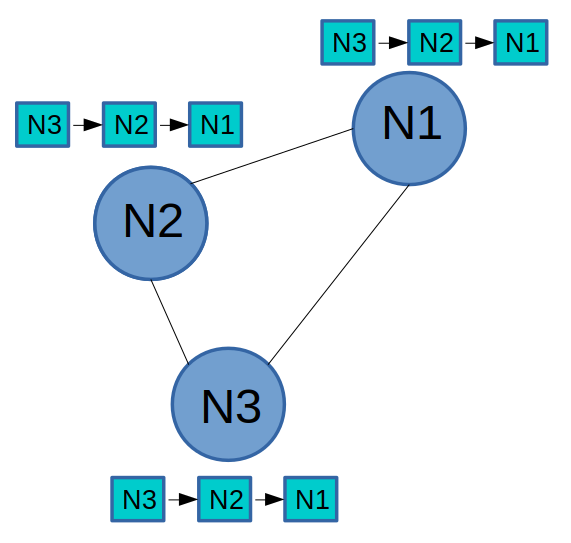
\includegraphics[scale=0.4]{network}
	\label{fig:network}
\end{figure}
\linebreak
\linebreak
But this design is not sufficient: a malicious peer can eavesdrop communication and be aware of the IDs of already joined peers. When a peer A leaves the network, a malicious peer M can usurpate A’s ID to communicate. If M manages to perform a man-in-the-middle attack, he can use A’s ID even when A is active by dropping its packets. We need authentication to prevent this. So we need to add another field in each block: the peer’s public key. This will allow each peer to verify that a peer claiming an ID is in posession of the corresponding private key and so is indeed the correct peer. This can be done with digital signatures either with a challenge-response protocol or with HMACs, we will explore this in the second part.
\linebreak
\linebreak
Here is a workflow of the joining protocol:
\begin{enumerate}
	\item A sends a rumor or private message m to B. We add a new field in every gossip packet : the node's ID.
	\item B sees that A’s ID is not part of the blockchain, so it sends to A an ID, a timestamp and the hash of the last block.
	\item A generates a public-private key pair.
	\item A mines a new block with the fields: ID, timestamp, pub\_key, nonce, prev\_hash
	\item A sends the block to B.
	\item B verifies it, if it is valid B adds the block to its local blockchain and broadcasts the new block using gossiping.
	\item B sends the whole blockchain to A and treats future gossip packets normally now that A is allowed to be part of the network.
\end{enumerate}
\begin{figure}[h]
	\caption{Block fields}
	\centering
	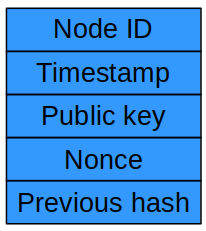
\includegraphics[scale=0.7]{block}
	\label{fig:block}
\end{figure}
At some later stage, in step 2, B will see that A is in the blockchain but the timestamp has expired. In this case the workflow is the same and we proceed with the same steps, which means A has to mine a new block again. This increases difficulty for an attacker to control a lot of peers: to have $N$ peers in permanence the adversary has to mine $N$ blocks every $\Delta t$ time units, where $\Delta t$ is the expiration delay.
\linebreak
We have to consider the case of bootstrapping a network: assume A and B are not joined in any network and want to communicate. A can make a join request to B as in step 1), then B will not proceed to step 2) since there is no blockchain yet. So B create its own block, the first of the blockchain (the genesis block, with any value as previous hash) and then it can proceed with step 2. In the gossiper command we add a new flag $genesis$ which can be set to true if the node wants to start the blockchain. It will consider itself joined only once it has mined the first block so only then other nodes will be able to join. To keep the design simple and avoid some problems, the genesis node is not considered a special node later, it behaves like the others which means its genesis block will expire at some point. So we assume that there is always at least one joined peer in the network, because otherwise the following can happen : node A mines the genesis block, no one tries to join and at some point the block expires, then B tries to join to A but A itself isn't joined anymore so no one can join anymore. This is the limitation of the design, but the assumption seems reasonable and if we set the expiration time large enough this is unlikely to happen.
\linebreak
Note that this does not handle merging of different peer-to-peer networks. One peer can join any network or create its own and wait for other peers to join, but a set of peers joined together cannot merge their blockchain with the one in another peer-to-peer network. We expect blockchains to diverge a lot in the network because nodes will try to join at the same time to different locations in the network. But actually we don't need to deal with collisions. If two blocks are mined concurrently, at each node one of them will simply be dropped. We will have 2 versions of the blockchain but that doesn't matter because nodes only need to be considered joined by their neighboring peers. We only needed to replace the node's ID field in every forwarded gossip packet so that for every incoming packet, the node's ID field is the one of a neighbor.
\linebreak
Moreover, we don't need to keep all blocks in the blockchain, we can remove the ones that expired. This does not affect the integrity of the blockchain because if one block expired, all previous blocks also expired So whenever a peer joins it receives the blockchain starting with the first valid block and not the others. The advantage is that we keep a blockchain that has always at most only $n$ blocks for a network of $n$ peers.
\subsection{P2P Authentication}
Once a peer has done a PoW it is registered in the blockchain and we must ensure that it can use this registration to communicate at any time before the block’s timestamp expires. Concretely if a node A leaves the network and comes back through some node B, it will present its ID and B will verify that the ID is present in the blockchain. Now we want to make sure that a malicious peer M cannot use A’s ID to communicate as A, so A signs every packet it sends to B with its private key. B can verify the authenticity and integrity of each packet with A’s public key which is present in the block with A’s ID.

This guarantees that A can connect to the network from any location at any time through any joined peer and that peer can verify that it is indeed A. But this is not enough because a malicious peer M could do a PoW and behave normally by connecting through B, and at the same time communicate normally through some other peers C, D, etc. Here we assume that the adversary has the means to communicate from different IP addresses to different peers. Each peer sees M behave normally but unless they share their information they will not realize that M has joined the network multiple times.

This is why we need to keep track of all the active nodes present in the network and share this information among all peers. Currently each peer knows its neighbor peers, but it must now know all the peers active in the network. To do this, each peer should maintain a local list of active peers and send to each of its neighbor a special packet whenever it allows a new peer to join the network. Whenever a peer receives such a packet from a neighbor it adds the new peer to its own list.
Now we have a way of sharing a list of all active nodes in the network but we need to be able to remove a peer from the list whenever it fails or leaves the network. For this we need nodes to regularly ping each other to check if they are still present. Luckily this is implicitly already done by the anti-entropy mechanism that sends status messages periodically. So we can determine that if after a period of time T a node A has not received any status messages from a neighbor B, A will consider B inactive and remove it from its list of active nodes. A will also broadcast in some special packet the information that B is now inactive. Upon reception of this packet, the other nodes will remove B from their list as well.

Now if the malicious peer M communicates through B, B will not only check the ID in the blockchain and the validity of the digital signature, it will also check that M is not already part of the list of active peers. If not B will allow M, add it to the list of active peers and propagate the change. Now if M wants to communicate through C, C  will not allow it since M is already part of the list of active peers.

To summarize, whenever a node A sends a first packet m to node B, B must perform the following checks :
1) Is A’s ID part of the blockchain ? If not proceed with the protocol in part1, If yes proceed to check 2
2) Is the signature of m valid using A’s public key present in the block ? If not reject m, if yes proceed to check 3
3) Is A already part of the list of active peers ? If yes reject m, if not add A to the list and propagate the information that A has joined to the neighbors, then treat m normally.

For the next packets, B only needs to check the signature.
\section{Evaluation}
We will create different p2p topologies and measure the joining time for a normal peer as well as the joining time for a set of Sybil peers in order to compare them. The normal joining time should be reasonable and the Sybil joining time should be very expensive. We will try different values for our parameters (the expiration delay and the difficulty of each cryptopuzzle) and compare the results.

We also have to check that coordinating multiple malicious peers will not affect the validity of the protocol. For example if a malicious peer wants to join through another malicious peer.

It is important to also make sure that bootstrapping of networks is done correctly (when no nodes are joined).
\printbibliography
\end{document}